\documentclass[main.tex]{subfiles}

\begin{document}
Due to uncertainties in how to deal with the gamma-beta sum spectrum, the central value of the Fierz term is not ready to be stated. 
However, most of the systematic effects can still be calculated.
The effect with the lower beta cut is likely due to the normalization of the beta-gamma sum spectrum.
The issue is a solvable one. 

\section{Discussion of Results}

The statistical uncertainty of $b_{gt}$ is 0.0042.
This is with 7 million events that pass the gamma coincidence.
If the lower beta cut uncertainty is excluded, the total systematic uncertainty is 0.0066.
This also excludes any uncertainty on the normalization of the gamma-beta sum spectrum.
This is dominated by the uncertainty on the weak magnetism.
If the lower beta cut uncertainty can be resolved, the total systematic uncertainty should only be a touch higher than 0.0066.
This is very close to the statistical uncertainty. 

To lower the systematic uncertainty, the weak magnetism should be known to a more precise value.
The uncertainty of the weak magnetism comes from how it is calculated.
The parameters need to calculated the weak magnetism are shown in equation \ref{eq:bwmcal} .
Most of the uncertainty comes from the gamma decay strength \cite{Min11}.
A better measurement of this gamma decay strength would reduce the effect of the weak magnetism.

\section{Results Compared to Other Measurements of the Fierz Term}

A similar measurement was done with ultra-cold neutrons \cite{Hic17}.
The beta decay spectrum was measured using a magnetic spectrometer.
The neutrons were confined in the center with a magnetic field, and allowed to decay.
A superratio was used to extract the Fierz term.
With the systematic effects, the final results of the Fierz term was $0.067 \pm 0.005_{stat}  ^{+0.090}_{-0.061} sys$.
Even with the lower beta cut effect, the systematic uncertainty of the Fierz term in the $^{20}$F measurement is much smaller.
The statistical uncertainty is comparable. 
Additionally, since the decay of a neutron is a mixed decay, this Fierz term is sensitive to both the tensor couplings and the scalar couplings.  
The beta spectrum is shown in figure \ref{fig:ucnabeta}.

\begin{figure}[!htb]
	\centerline{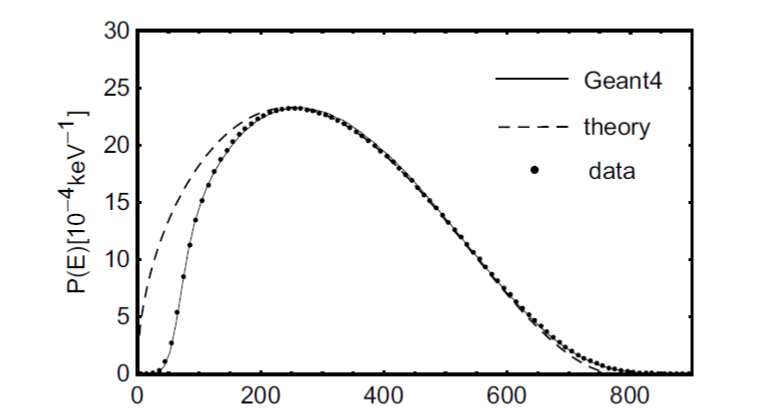
\includegraphics[width=0.78\textwidth]{NeutronBetaSpectrumUCNA.png}}
	\caption{The energy spectrum of the ultra-cold neutron measurement \cite{Hic17}}
	\label{fig:ucnabeta}
\end{figure}

There are large distortions at low energy due to back-scattering effects. 
The systematic uncertainty quoted due to backscattering effects is $\pm 0.005$, which is larger the statistical uncertainty of this $^{20}$F measurement.
The largest systematic uncertainty in the neutron measurement was due to uncertainties in the detector calibration.
The fluorine measurement avoids this, as the gain is left as a free parameter.

Another method to get the Fierz term is by measuring $ft$ values.
From the superallowed beta decays, the result for the Fierz term is $-0.0028 \pm 0.0026$ \cite{Har17}.
It was obtained with $ft$ vaule measurements of 14 different nuclei. 
The uncertainty is the statistical uncertainty of the fit after the $ft$ values were corrected.
However, this Fierz term is sensitive to scalar couplings, and not tensor coupling like in the $^{20}$F measurement.
It had different systematic effects, and it took 14 different measurements to come up with this number.
Even with all this, the potential sensitivity to the implant technique is similar to that of 14 $ft$ value measurements.

A different measurement with sensitivity to tensor couplings was made with $^{60}$Co \cite{Wau10}.
This measurement measured the beta asymmetry.
Then, this asymmetry was compared to the standard model value.
This was done with a large magnet. 
The largest uncertainty was due to the size and location of the source.
The limit on the tensor couplings was between $-0.089$ and $0.013$.
Assuming that $C_{A}' = 0$, this corresponds to a similar error bar in the Fierz term.
This uncertainty is larger than the uncertainty due to the lower beta cut effect.

In order to compare this to high energy techniques, equation \ref{eq:bgtpropor} is used \cite{Gon19}.
If the lower beta cut effect is resolved and the systematic effects described above accurate, then the total uncertainty on $b_{gt}$ is 0.0055. 
This corresponds to an uncertainty on $Re(\epsilon_{t}$ of 0.0009.
This is twice the uncertainty from the neutral current channel at the LHC. 
However, to reach this uncertainty, all that would be needed would be to run the the experiment again with higher statistics. 
Then, the statistical uncertainty would be negligible, and the systematic uncertainty would be the limiting factor. 

\section{Further Refinements to Technique}
The first thing to do to improve the experiment is to run more events.
Most of the events ran for this experiment were with the PVT detector.
However, the shape of beta spectrum in that detector had an odd distortion in it.
If that could be investigated and solved, using a plastic scintillator would be an ideal candidate for this measurement.
Less of the gamma ray would be absorbed, and there would be less bremmstrahlung in the detector.

The largest systematic effect right now is the lower beta cut effect. 
This can probably be solved by adjusting the normalization of the gamma-beta sum spectrum compared to the implant detector. 
This has to be seen that it works properly with Monte Carlo.
Ultimately, the resulting offset and sum spectrum level probably are not the real, physical level.
Tuning them on the stability of the results relative to the lower beta cut does give reasonable answers.
Then, an estimate of the uncertainty to the offset and the level of the gamma-beta sum spectrum would have to be done.
The offset is likely known to 0.5 and the level likely to 10\%.
This would likely be the largest systematic uncertainties.
As these uncertainties depend on the slopes of the lower beta cut curves, these should get more precise as more events are built.
The slope can be seen more easily as there is the error bars get smaller.

The gamma-beta sum spectrum is a trickier. 
If the slope of the $b_{gt}$ is used, then at higher statistics, the same reduction could occur. 
Another method would be to compare the output of GEANT4 to that of another simulation code.
This was done with EGSnrc, and agreement was found to <AGREEMENT VALUE>.
Other packages and processes would be good.

In order to increase efficiency for the 1.6 MeV gamma ray, the implant detector could be more completely encased with gamma detectors.
If these gamma detectors had a higher resolution, that would mean that the signal in the implant would be much cleaner.
If that were coupled with a plastic detector, then the beta spectrum of the implant detector would be much cleaner.
This would hopefully eliminate the amount of gamma-beta sum spectrum.

If these systematic effects are reduced, the next largest one has to do with the uncertainty on the measurement of $b_{wm}$.
There, a new and better measurement of the transition strength in $^{20}$Ne would have to be measured.
Increasing the precision on the energy of the gamma rays would help both with the electron maximum energy and with the $b_{wm}$.
This would require a different type of experiment.

\section{Conclusion}
With all this in place, this measurement of the Fierz term can be one of the more precise ones, if the issue with the lower beta cut can be figured out.
Many of the systematic effects would be present in other such measurements.
This measurement can be competitive with high energy measurements, but it took much less equipment.


\end{document}
